%%%%%%%%%%%%%%%%%%%%%%%%%%%%%%%%%%%%%%%%%%%%%%%%%%%%%%%%%%%%%%%%%%%%%%%%%%%
%% This file is part of the book
%%
%% Algorithmic Graph Theory
%% http://code.google.com/p/graph-theory-algorithms-book/
%%
%% Copyright (C) 2009--2011 Minh Van Nguyen <nguyenminh2@gmail.com>
%%
%% See the file COPYING for copying conditions.
%%%%%%%%%%%%%%%%%%%%%%%%%%%%%%%%%%%%%%%%%%%%%%%%%%%%%%%%%%%%%%%%%%%%%%%%%%%

\documentclass{article}

\usepackage{tikz}
\usetikzlibrary{external}
\tikzexternalize{digraph-flow}

\begin{document}

\begin{figure}
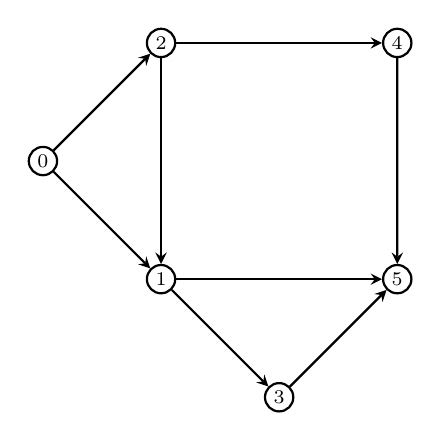
\begin{tikzpicture}
[nodeDecorate/.style={shape=circle,inner sep=1.5pt,draw,thick},%
  arrowDecorate/.style={->,>=stealth,thick},%
  scale=1.5]
\scriptsize
%% nodes or vertices
\foreach \nodename/\x/\y in {0/0/0, 1/1/-1, 2/1/1, 3/2/-2, 4/3/1, 5/3/-1}
{
  \node (\nodename) at (\x,\y) [nodeDecorate] {$\nodename$};
}
%% edges or lines
\path
\foreach \startnode/\endnode in {0/1, 0/2, 1/3, 1/5, 2/1, 2/4, 3/5, 4/5}
{
  (\startnode) edge[arrowDecorate] node {} (\endnode)
};
\end{tikzpicture}
\end{figure}

\end{document}
